\documentclass[a4paper,12pt]{article}
\usepackage{a4wide}
\usepackage{natbib}
\usepackage{graphicx}
\usepackage{color}
\usepackage{listings}

\usepackage{hyperref}
\hypersetup{
    bookmarks=true,         % show bookmarks bar?
    unicode=false,          % non-Latin characters in Acrobat’s bookmarks
    pdftoolbar=true,        % show Acrobat’s toolbar?
    pdfmenubar=true,        % show Acrobat’s menu?
    pdfnewwindow=true,      % links in new window
    colorlinks=true,       % false: boxed links; true: colored links
    linkcolor=blue,          % color of internal links
    citecolor=green,        % color of links to bibliography
    filecolor=magenta,      % color of file links
    urlcolor=cyan           % color of external links
}

\title{\vspace{-4cm}Turku Event Extraction System\\}
\author{}
\date{}

\begin{document}

\maketitle

\vspace{-2cm}\begin{description}
%\item[Software:] University of Turku BioNLP'09 Event Detection Software
\item[Release Date:] 25.03.2010
\item[Version:] 1.0
\item[Authors:] Jari Bj{\"{o}}rne, Juho Heimonen, Filip Ginter, Antti Airola,
Tapio Pahikkala and Tapio Salakoski
\item[Contact:] Jari Bj{\"{o}}rne (jari.bjorne@utu.fi)
\end{description}

\tableofcontents

\section{Introduction}

This software package contains the system designed to detect biomedical events as
defined in the BioNLP'09 Shared Task. It combines machine learning and rule based
systems, using Joachims SVM-Multiclass for the machine learning components.

This release contains software required for detecting events as
defined in the tasks 1, 2 \& 3 of the shared task, starting from textual data in
the interaction XML (see section 5) format. Software is also provided for
generating the XML from the BioNLP'09 Shared Task data format.

This file describes the overall design and use of the event extraction system.
For the API documentation, see doc/index.html.

\section{Related Publications}

This release covers the following publications:

\vspace{5 mm}

J. Bj{\"{o}}rne, F. Ginter, J. Heimonen, S. Pyysalo, and T. Salakoski. Learning to
extract biological event and relation graphs. \emph{In Proceedings of the 17th
Nordic Conference on Computational Linguistics (NODALIDA’09)}, 2009.
\url{http://portal.acm.org/citation.cfm?id=1572343}

\vspace{5 mm}

J. Bj{\"{o}}rne, J. Heimonen, F. Ginter, A. Airola, T. Pahikkala, and T.
Salakoski. Extracting complex biological events with rich graph-based feature
sets. \emph{In BioNLP ’09: Proceedings of the Workshop on BioNLP, pages 10–18,
Morristown, NJ, USA, 2009. Association for Computational Linguistics. ISBN
978-1-932432-44-2}, 2009. \url{http://portal.acm.org/citation.cfm?id=1572343}

\vspace{5 mm}
   
J. Bj{\"{o}}rne, J. Heimonen, F. Ginter, A. Airola, T. Pahikkala, and T.
Salakoski. Extracting o contextualized complex biological events with rich
graph-based feature sets. \emph{Computational Intelligence, Special issue on
Extracting Bio-molecular Events from Literature}, 2010. To appear.

\section{Overview of the Software}

The design of the system aims to separate and abstract the machine learning away
from the actual textual data. In this, the system follows traditional machine
learning approaches where all kinds of data are handled through a generic feature
vector representation. The learning component is a thin wrapper around the
SVM-multiclass classifier, and can be replaced with other learning systems. Most
the components are independent, so different components can be mixed to perform
different experiments.

The event detection approach is based on first detecting \emph{triggers}, words
such as ``bind'' or ``phosphorylate'' that define interactions
(Figure~\ref{fig-sentence}C). Event argument \emph{edges} are then predicted
between the triggers and \emph{named entities} (Figure~\ref{fig-sentence}D).
The resulting graph is processed into a format that explicitly defines the full
nested event structures (Figure~\ref{fig-sentence}E). This graph can finally be
converted into the BioNLP'09 Shared Task format.

The event detection requires sentences to be parsed sentences and named
entities (usually gene or protein names) to be marked. For parsing and named
entity detection, other software must be used (Figure~\ref{fig-overview}).

\begin{figure}[h]
\begin{center}
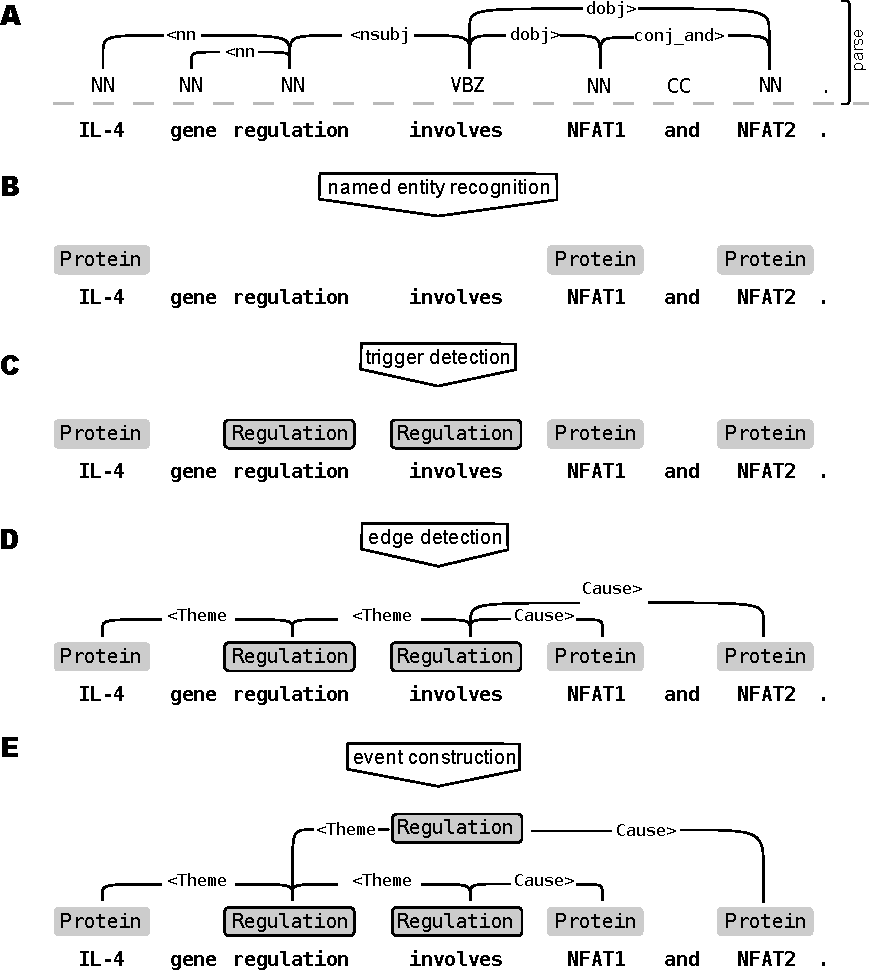
\includegraphics[scale=0.75]{Figures/model-sentence-pubmed1p.pdf}
\end{center}
\caption{The event detection approach.}
\label{fig-sentence}
\end{figure}

\begin{figure}[h]
\begin{center}
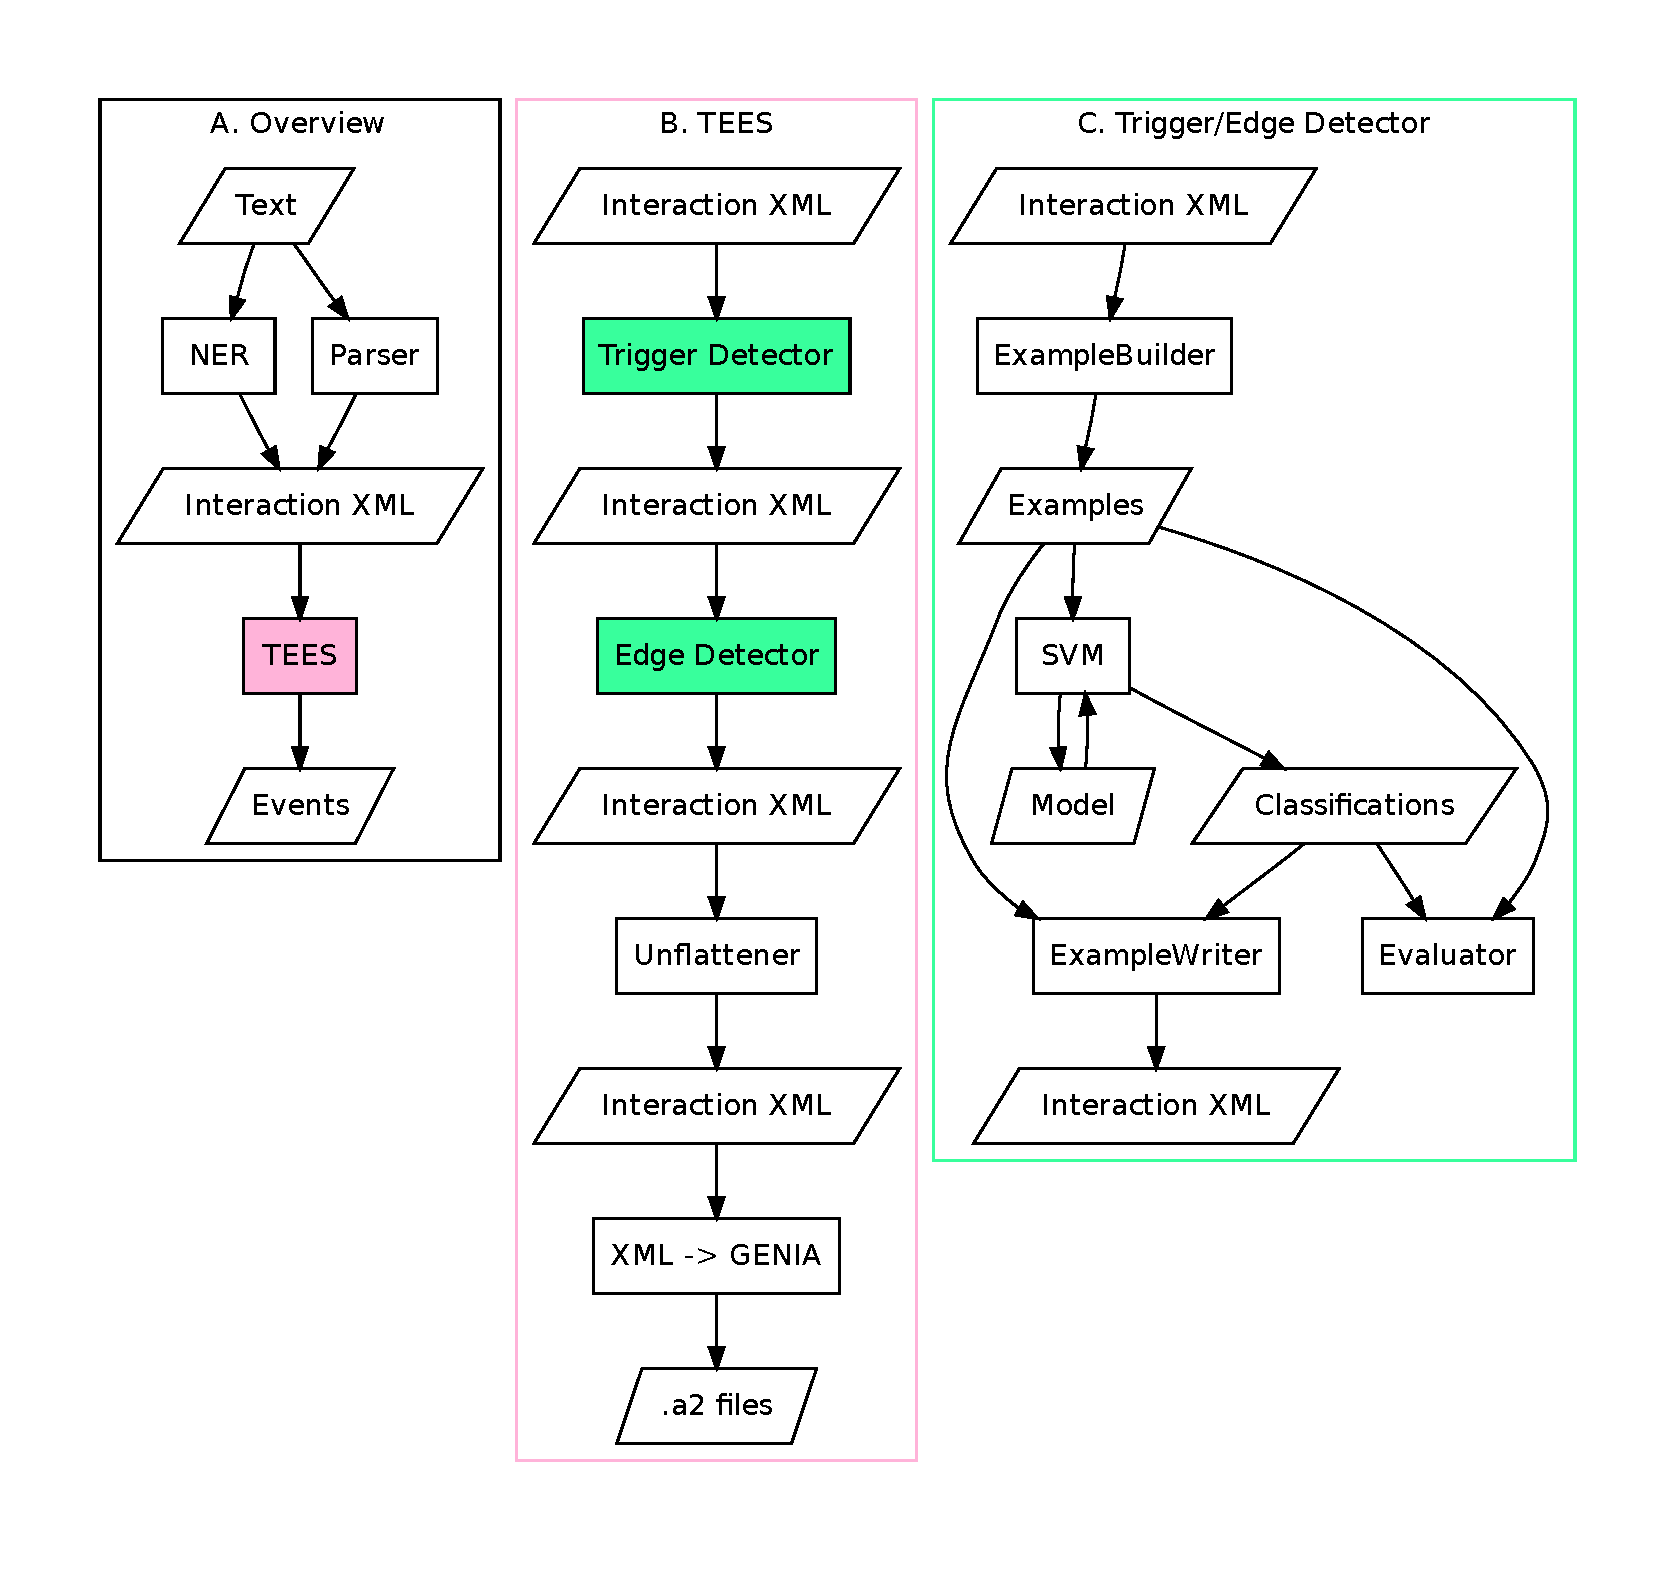
\includegraphics[scale=0.5]{Figures/overview.pdf}
\end{center}
\caption{The Turku Event Extraction System (TEES) detects events
in parsed sentences which have annotated named entities, or where named
entities have been detected with a named entity recognizer (NER).}
\label{fig-overview}
\end{figure}

The BioNLP'09 Shared Task data provides parses and named entities. We provide
this data already in the interaction XML format. It should be quite simple to
insert e.g. your own parses into this format. In case you need to rebuild your
own interaction XML files, use XXX.

\section{How to Use It}

For most cases, the steps for using the software are:

\begin{enumerate}
  \item Reoptimize the parameters (only if training data has changed).
  \item Regenerate the SVM model files (only if training data has changed).
  \item Classify your test data using the SVM model files.
\end{enumerate}

\subsection{Required Software \& Hardware}
\label{sec-requirements}

The main requirement of the software is Python, at least versions 2.4 and 2.5 are
known to work. Additionally, if you want to use the BioNLP'09 official evaluation
tools, you will need to have perl installed, and have it in the PATH and callable
with the command "perl".

For additional settings, there is a settings file located in src/Settings.py. You
probably only need to modify it if you want to retrain the system, in which case
you need Joachims SVM-multiclass. Download it from
\url{http://svmlight.joachims.org/svm\_multiclass.html} and compile with a C
compiler. You will now have two binaries, "svm\_multiclass\_learn" and
"svm\_multiclass\_classify". In src/Settings.py set the variable SVMMultiClassDir
to point to the directory containing the binaries.

All the included XML-files contain information for all three subtasks of the
BioNLP'09 Shared Task. All the model files are trained for joint prediction of
tasks 1 \& 2. Results for the primary task 1 can be obtained by giving the
correct task parameter for the relevant pipeline.

Classification of the Shared Task dataset can take more than 1 Gb of memory, but
the system should run fine on a machine with at least 2 Gb.

\subsection{Running the System}
\label{sec-running}

The system is controlled by writing "pipeline files", which are simply Python
scripts that call functions defined in the public interface of the event
detection system. These functions usually pass the same data forward, each
performing some step in the experiment. There are multiple pre-made pipelines in
the package, and these should cover the most common use cases of the software.
These are located in src/Classifiers/. To run a pipeline, simply call it with
python "python name.py". For the provided pipelines, you can also pass command
line parameters. To see a list of available options, call the program with the
option "$--$help".

The BioNLP'09 Data used for training and testing the system is divided into
four sets. \emph{Train} and \emph{devel} sets are both known data, and are used
to e.g. optimize parameters. The \emph{everything} set is a union of train and
devel sets and is used to maximize the amount of training data when classifying
the hidden \emph{test} set (Figure~\ref{fig-sets}).

\begin{figure}[h]
\begin{center}
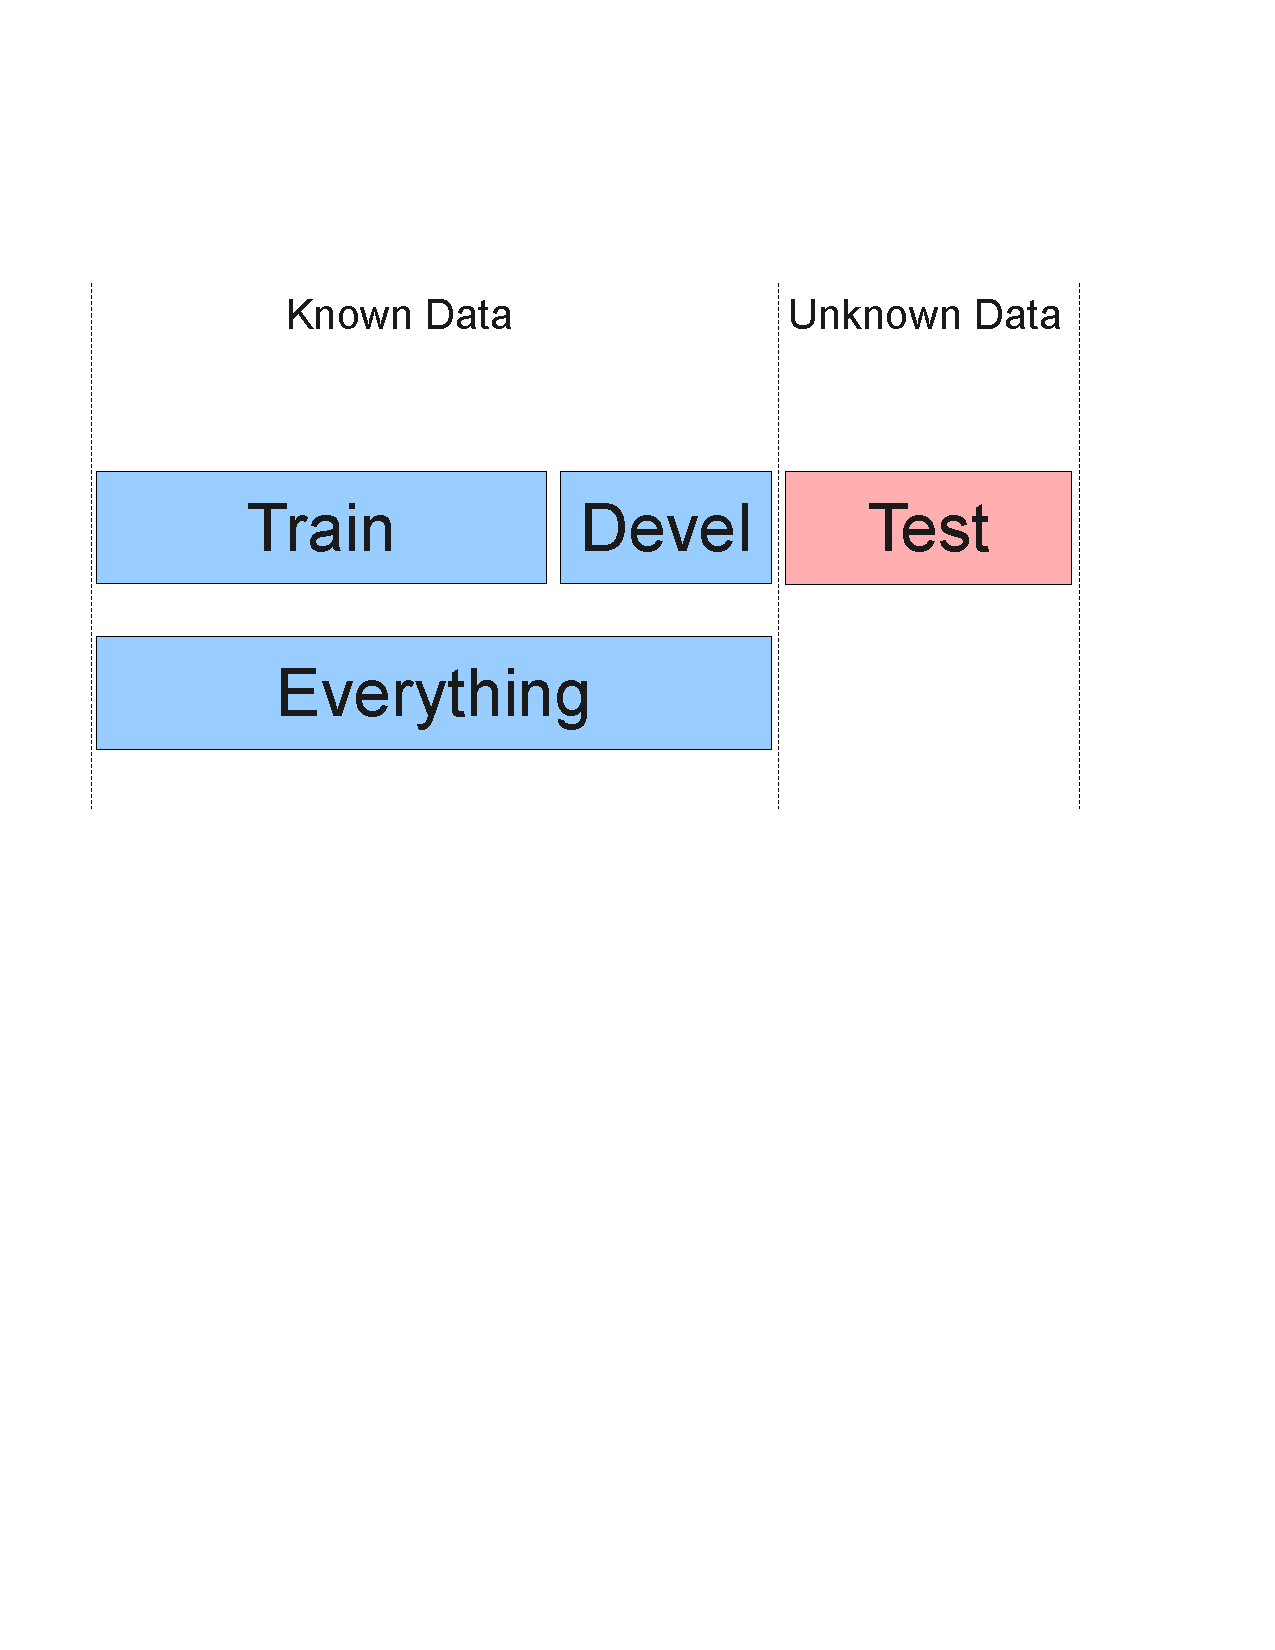
\includegraphics[trim = 0mm 150mm 0mm 50mm,
clip,scale=0.5]{Figures/DataSets.pdf}
\end{center}
\caption{The BioNLP'09 data sets.}
\label{fig-sets}
\end{figure}

\subsection{Quick Start (test basic classification)}

\begin{enumerate}

\item Create an empty directory for the program output, e.g. /OUTPUT.

\item Go to directory src/Pipelines.

\item Execute the command "python BioNLP09Classify.py -o /OUTPUT". The program will
perform event detection on the BioNLP'09 Shared Task devel-set, using pre-defined
learned information from the Shared Task train set.

\item The program will print progress information on screen. If you haven't set up
SVM-multiclass, classification will work but will be very slow.

\item Final results will show on screen using the official shared task evaluation
script. The output directory will contain a "geniaformat" subdirectory with the
predicted ".a2" files.

\end{enumerate}

\subsection{Classifying with Pre-trained Models (Task 1 \& 2)}

For using the pre-trained models for classification, use
src/Pipelines/BioNLP09Classify.py. The program has many parameters, but the
simplest test run takes just one, "-o" for the output directory which will be
created if it doesn't exist. Running like this will classify the BioNLP'09 Shared
Task devel set, for which you get the full set of available evaluations,
including the official shared task evaluation, as described in
section~\ref{sec-running}.

Classification will work even without SVM-multiclass, but is extremely slow
(slightly faster if you have numpy installed). See
section~\ref{sec-requirements} for instructions on how to download and configure SVM-multiclass.

If you have made your own input interaction xml file (such as a new corpus or
something), and just want to classify it with our models, use the "-i" parameter
to define that file. You can also use "-t" and "-p" to define a tokenization and
parse, but remember that the system is using models trained on our parses, so if
yours differ too much, performance will suffer.

If you have re-trained the system (see Section~\ref{sec-retraining}), you can
use "-m" and "-n" to point to the model files, and "-r" to define your optimal 
recall adjuster parameter.

\subsubsection{Important note on feature and class ids}

If you have modified the provided training files, or are using some other data
for training, the examples generated from it may contain new features. The
support vector machine has no knowledge of the feature and class names, and
instead uses integer ids to represent them. When given something to classify, it
will match classes and features based on these ids. Therefore it is extremely
important that the ids are consistent between training and classification.

When retraining the system, new id files are created in the output directory.
These are of the format STEM.class\_names and STEM.feature\_names. When using
your new models (with the "-m" and "-n" parameters), remember to also use the
matching id sets with the "-v" and "-w" parameters.

\subsection{Retraining the system}
\label{sec-retraining}

\begin{figure}[h]
\begin{center}
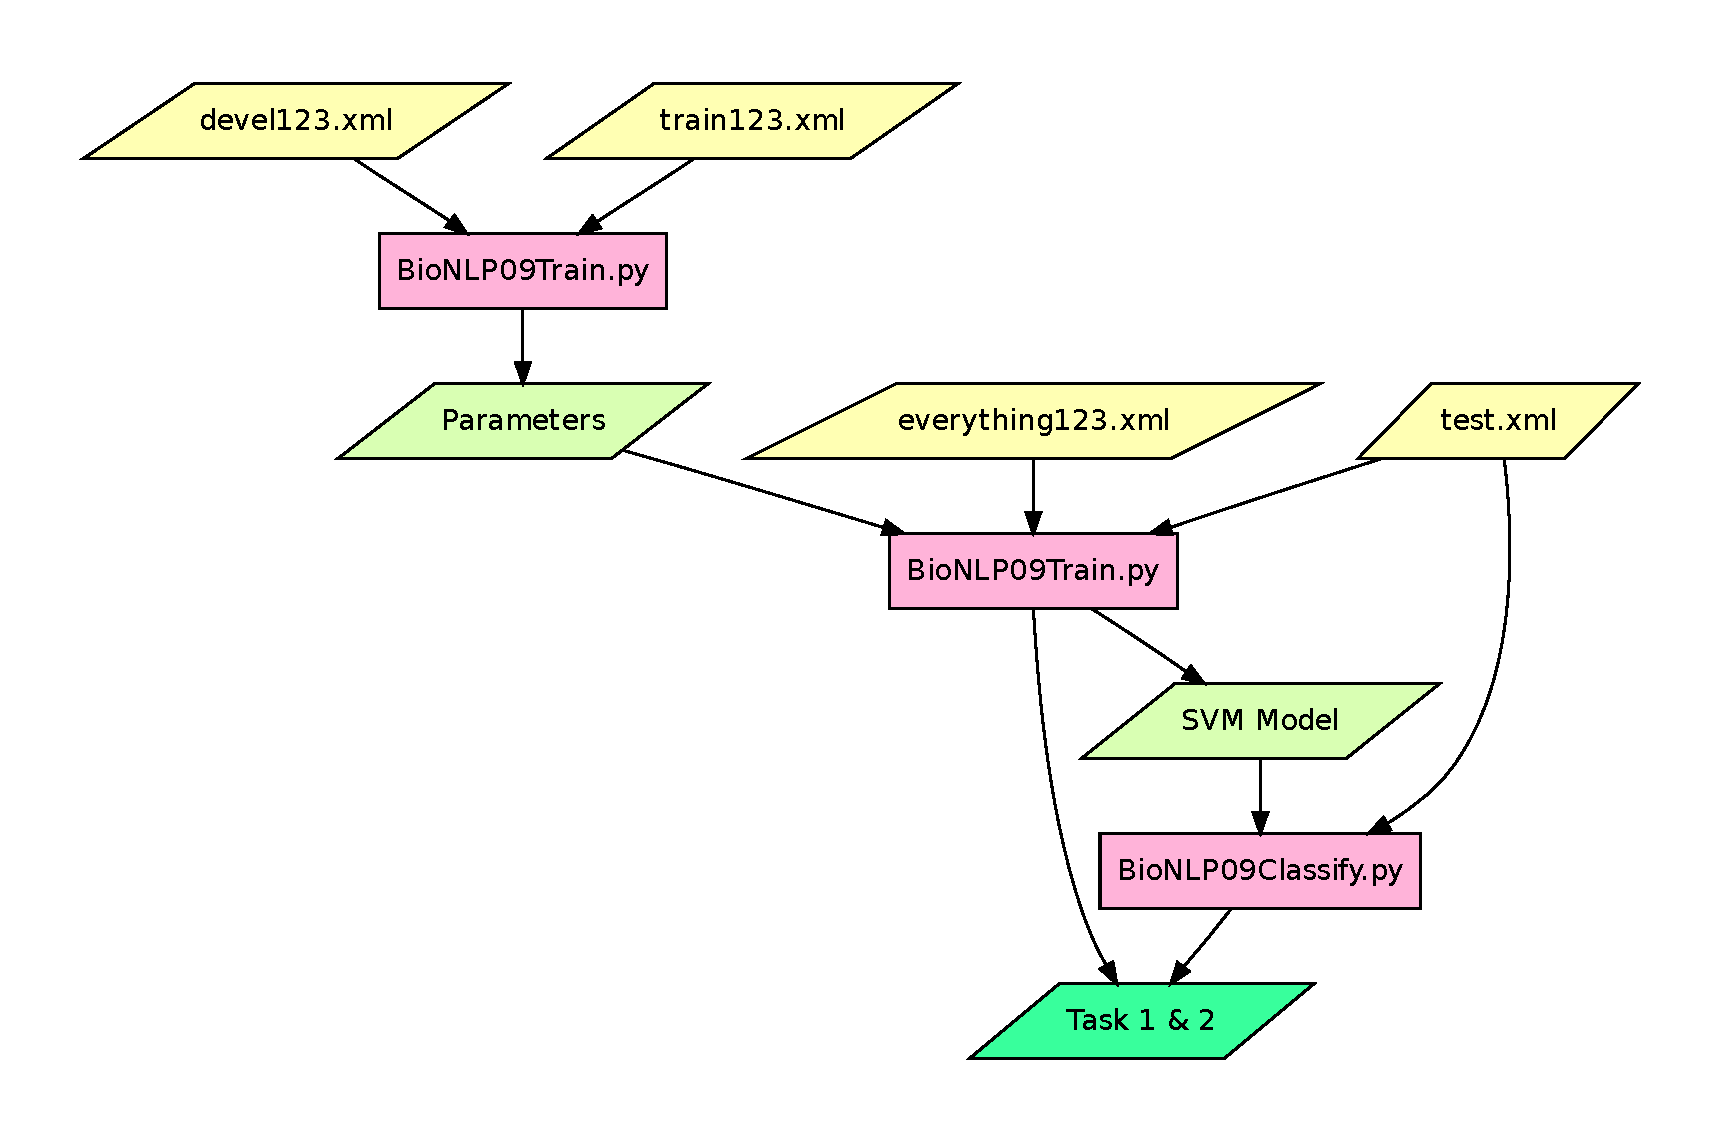
\includegraphics[scale=0.5]{Figures/programs12.pdf}
\end{center}
\caption{BioNLP09Train.py is used to build SVM models from the training data
(train or everything) and to search for the optimal parameters using known data
(devel). With pre-generated models, BioNLP09Classify.py can be used to directly
classify test data. }
\label{fig-programs12}
\end{figure}

If you modify the training data (such as using a new parse) or use a new dataset,
you must retrain the system. For retraining, use src/Pipelines/BioNLP09Train.py
(Figure~\ref{fig-programs12}). The retraining proceeds in two steps. First, one
SVM model is created for each trigger and edge c-parameter to be tested. Then, using these models, triplets of
trigger c-parameter, edge c-parameter and recall booster parameter are tested in
the three-dimensional search space to determine the optimal parameter
combination. The program will print evaluation results for all combinations on
screen. This output is also stored for later use in a file called log.txt in the
output directory.

The program has several options. Options "-e" and "-r" are used to to define your
training and testing files. The SVM uses training data to learn its
classification principles, and testing data for determining the optimal
regularization parameter c. Both files are in Interaction XML format, more
information on which can be found in section 5.

Output directory "-o" will be created if it doesn't exist. If you have created
new parse and tokenization elements in the interaction xml files, they can be
used with the "-p" and "-t" options. Id sets ("-v" and "-w") should use the
default values, so most features will be consistent with the pre-defined models.

The three parameters to optimize can be defined with options "-x" (trigger
detector c-parameter), "-y (recall booster parameter)" and "-z" (edge detector
c-parameter). All of these take as input a comma separated list of numbers,
integers in the case of "-x" and "-z" and floats for "-y". Determining good
parameter ranges for optimization is somewhat a case of trial and error, but the
provided default values should be good for most situations. The SVM
regularization parameters, or c-parameters, can be almost anything, but for this
system usually exist in the range of 10000--1000000.

The recall booster parameter is used to multiply the SVM's prediction strength
for the negative class for each trigger. Therefore, recall booster parameters
$<$1 cause more potential triggers to be classified as actual triggers and increase
the recall. Parameters $>$1 reduce the number of triggers and increase
precision.

When re-training the system, two things must be kept in mind when looking for the
optimal parameter combination. First, the three-dimensional search grid must be
dense enough. Second, if an optimal parameter triplet is discovered on the edge
of the grid, it is possible that even better values are left outside the search
space, and increasing the grid in the direction of the parameter(s) on the edge
is recommended.

\subsection{Task 3}

Task 3 is about detecting whether events are stated in a speculative or
negative manner. Therefore task 3 requires predicting these attributes for
already existing events, and so happens outside the main event detection
sequence. A predicted event file (with task 1 or 2 events) can be used as input
for task 3 classification with src/Pipelines/BioNLP09ClassifyTask3.py
(Figure~\ref{fig-programs3}). 

For retraining the task 3 system, use src/Pipelines/BioNLP09TrainTask3.py, in a
similar approach as for tasks 1 \& 2. It is important to use the
duplicate-containing versions of the interaction XML files for task 3
experiments, as these are the files where the events are fully represented in the
graph. When predicting task 3 over task 1 or 2 predictions, the
"test-predicted-edges-unflattened.xml" output file from BioNLP09Classify.py is in
the correct, duplicate-containing format.

\begin{figure}[h]
\begin{center}
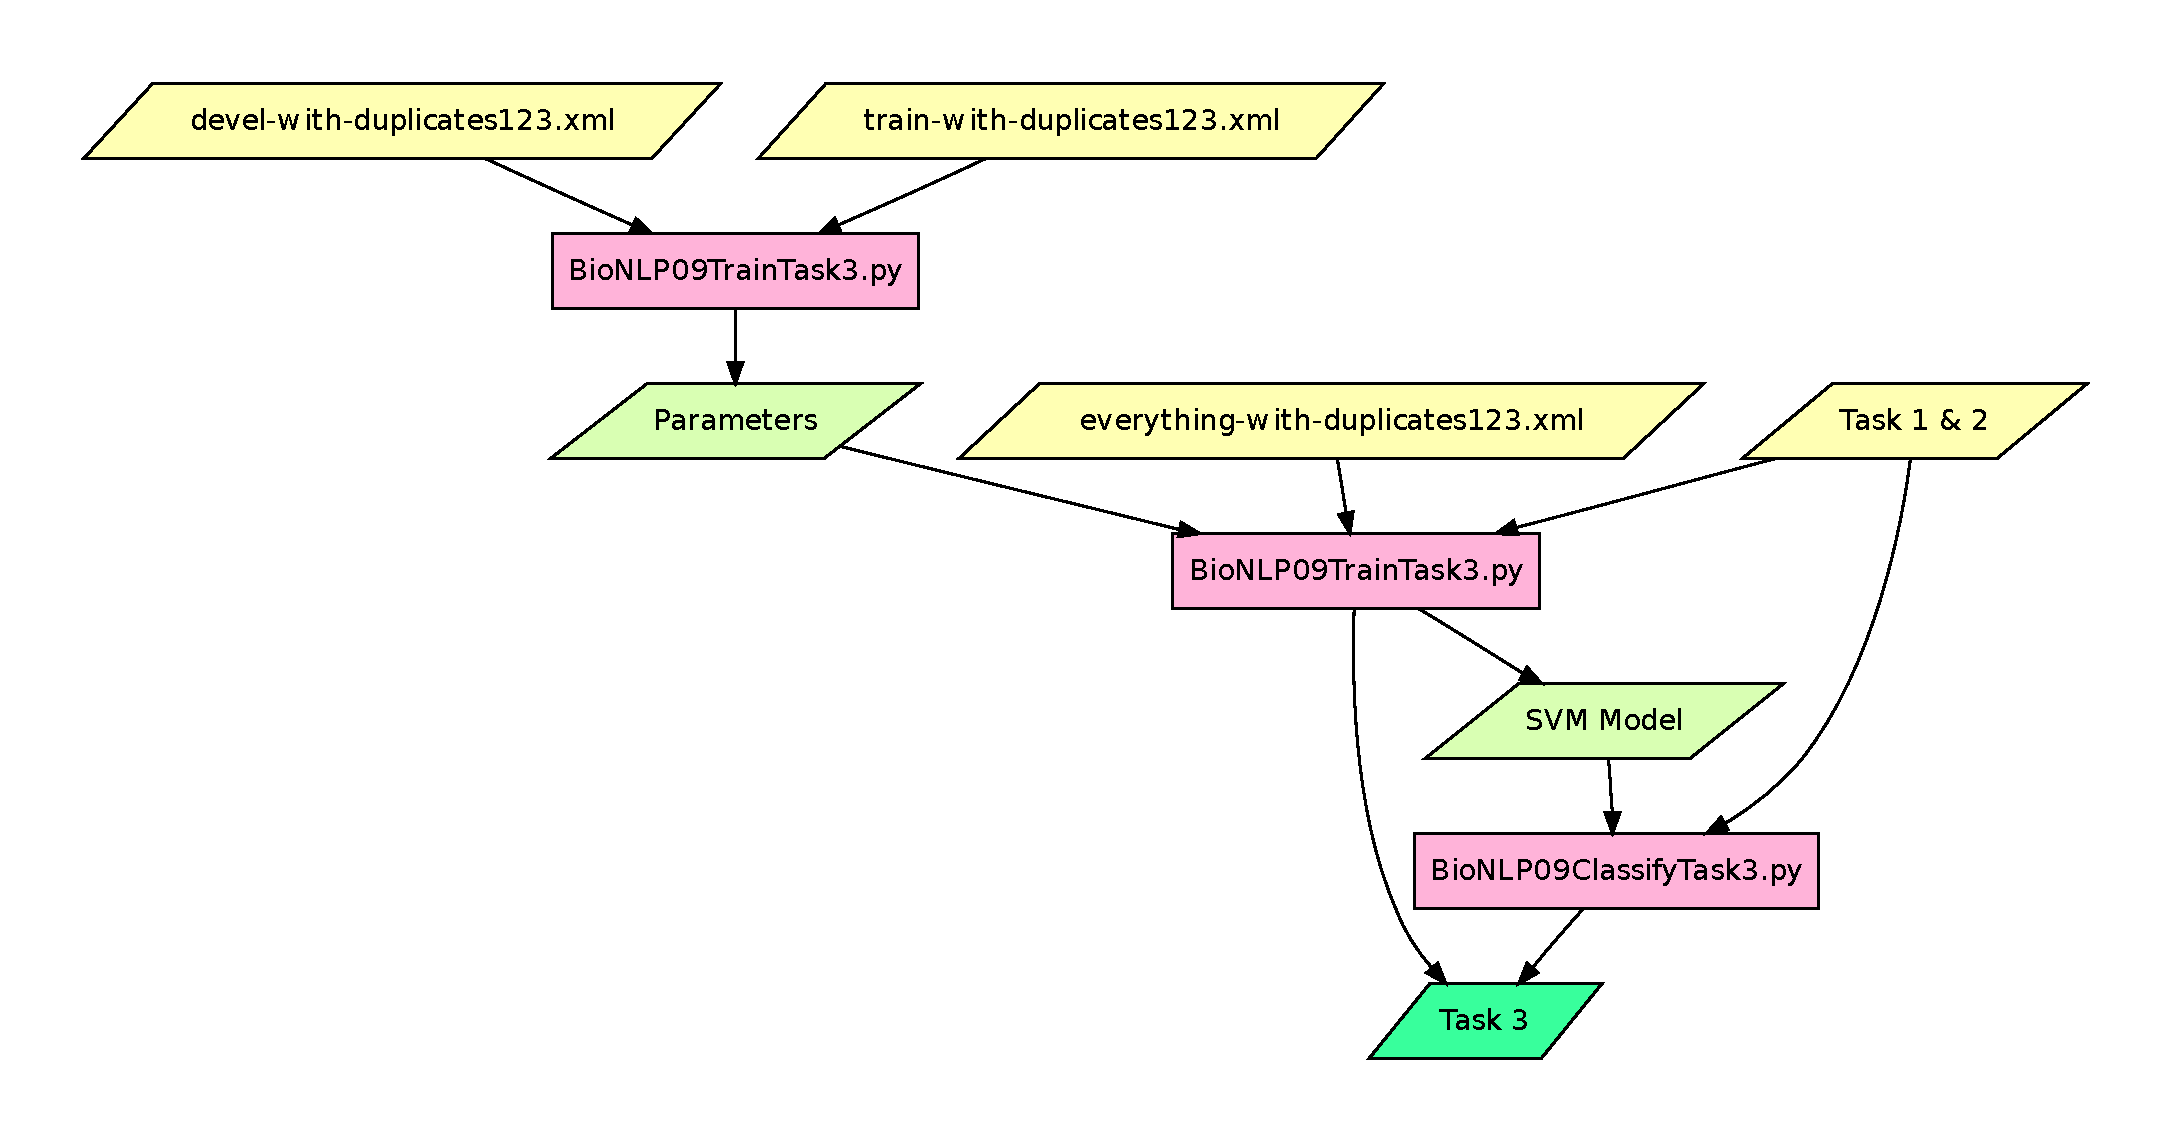
\includegraphics[scale=0.5]{Figures/programs3.pdf}
\end{center}
\caption{BioNLP09Train.py is used to build SVM models from the training data
(train or everything) and to search for the optimal parameters using known data
(devel). With pre-generated models, BioNLP09Classify.py can be used to directly
classify test data.}
\label{fig-programs3}
\end{figure}

\subsection{Writing Your Own Pipelines}

The file src/Pipelines/Pipeline.py defines the public interface of the event
detector. Following the example of the pipelines introduced above, you can
also write your own to make different experiments.

\section{Interaction XML}

\subsection{Corpus Files}

Interaction XML is the graph format used for representing the Shared Task data.
It is semantically equal to the shared task format, but when training for event
detection, it is compressed into a "flat/merged" format (See the BioNLP'09
publication). The corpus files provided in this package are already in the flat
format. The files are:

\begin{itemize}
\item /data/devel123.xml: Shared Task devel set with information for all three tasks

\item /data/train123.xml: Shared Task train set with information for all three
tasks 

\item /data/everything123.xml: Combination of the devel and train sets, used
for training when classifying the test set

\item /data/test.xml: Shared Task test set, no annotation available. The Shared
Task organizers provide an online evaluation system
\footnote{\url{http://www-tsujii.is.s.u-tokyo.ac.jp/GENIA/SharedTask/eval-test.shtml}}.

\end{itemize}

For converting XXX.
However, for most applications, the interaction xml files provide the best
starting point. For example, if you want to use a new parse, just insert it into
the interaction xml files, and it can be immediately used with the event
detection system.

\subsection{Format}

The interaction xml is an xml format describing sentences, their semantic content
and (optionally) automated analyses such as parses. It was originally
developed as a shared format for unifying a number of binary interaction corpora
\footnote{\url{http://mars.cs.utu.fi/PPICorpora/}}, but can be used as is for
representing also event-type complex interactions. It is extensible, and new
elements and attributes can be defined as long as their names don't overlap with existing
ones. Here is an example of the format, with one instance of all elements:

\lstset{% general command to set parameter(s)
language=XML,                % choose the language of the code
showspaces=false,               % show spaces adding particular underscores
showstringspaces=false,         % underline spaces within strings
numbers=left,                   % where to put the line-numbers
basicstyle=\small, % print whole listing small
stringstyle=\color[rgb]{0.5,0.5,1},
%keywordstyle=\color[rgb]{0,0,1},
%tagstyle=\color[rgb]{0,0,1},
%commentstyle=\color[rgb]{0.133,0.545,0.133},
%stringstyle=\color[rgb]{0.627,0.126,0.941},
frame=single,	                % adds a frame around the code
breaklines=true                % sets automatic line breaking
} % no special string spaces

\begin{lstlisting}
<corpus source="GENIA">
  <document id="GENIA.d0">
    <sentence charOffset="0-168" id="GENIA.d0.s0" origId="10089566.s0" text="Involvement of adenylate cyclase and p70(S6)-kinase activation in IL-10 up-regulation in human monocytes by gp41 envelope protein of human immunodeficiency virus type 1.">
      <entity charOffset="37-50" headOffset="37-39" id="GENIA.d0.s0.e0" isName="True" negation="False" origId="10089566.T1" speculation="False" text="p70(S6)-kinase" type="Protein" />
      <interaction directed="True" e1="GENIA.d0.s0.e1" e2="GENIA.d0.s0.e4" id="GENIA.d0.s0.i0" origId="10089566.E1.0" type="Theme" />
      <sentenceanalyses>
        <tokenizations>
          <tokenization tokenizer="McClosky">
            <token POS="NN" charOffset="0-10" id="clt_1" text="Involvement" />
 	</tokenizations>
        <parses>
          <parse parser="McClosky" tokenizer="McClosky">
            <dependency id="clp_1" t1="clt_4" t2="clt_3" type="nn" />
	  </parse>
	</parses>
      </sentenceanalyses>
    </sentence>
  </document>
</corpus>
\end{lstlisting}

The XML format defines a corpus, that contains sentences grouped into documents.
In the case of GENIA, these documents represent article abstracts. For each
sentence, a number of entities and interactions are defined. The entities
represent the named entities and triggers of the events, the interactions their
arguments (Theme/Cause etc.). The entities and interactions define the semantic
network (see BioNLP'09 article).

Character offsets are defined in the \emph{offset}-attributes, all offsets are
zero based (e.g. the offset of "A" in the beginning of the sentence would be "0-0").
Entity offsets are relative to the sentence, sentence offset is relative to the
document. The sentence's \emph{origId} attribute defines its GENIA/PubMed
identifier.

Entities represent both the named entities and trigger words of the events. The
\emph{isName} attribute must be \emph{True} for named entities, \emph{False} for triggers.
Attributes \emph{speculation} and \emph{negation} are specific for task 3 of the Shared
Task. The \emph{headOffset} attribute defines the syntactic head of the entity. This
is always based on a specific parse, see section~\ref{sec-editing}.

Interactions are the edges of the semantic network, and correspond to event
arguments. They are directed from entity one (e1) to entity two (e2). The
directed attribute is optional, if present it must be "True" for event detection.

The optional sentenceanalyses-element contains the parses. All parses consist of
a tokenization/parse pair. Tokens should be listed in the order they appear in
the sentence, and their ids must be of the format NAME\_x, where NAME is any
string and x is a number in the range [1,n]. Dependencies don't require ids, but
if they are used, they must be unique. The parses are identified with the
\emph{parser} and \emph{tokenizer} attributes. Most of the event detector components
allow also giving only the parse name as input, and for this reaseon each parse must
have a tokenizer-attribute defining the corresponding tokenization.

The format uses mostly hierarchical ids. These are the ids of documents
(NAME.d0), sentences (NAME.d0.s0), entities (NAME.d0.s0.e0) and interactions
(NAME.d0.s0.i0). Their numbering starts from 0 and for each element its
corresponding number must be unique. For fixing or updating these numbers, the
Pipeline command ix.recalculateIds can be used. This can also be done
externally with the program at src/CommonUtils/InteractionXML/RecalculateIds.py.

\subsection{Notes on Editing the Corpus Files}
\label{sec-editing}

To perform your own experiments, you will need to modify the interaction xml
files provided in this package. A single interaction xml can have multiple parse
and tokenization elements, as long as they have different \emph{parser} and
\emph{tokenizer} attributes.

Remember to keep the hierarchical ids valid, and use
src/CommonUtils/InteractionXML/RecalculateIds.py to fix them if in doubt.

For event detection, all entities are mapped to the parse through a single head
token (see BioNLP'09 article). This is defined as the "headOffset" attribute of
the entity. When you want to use a different parse, these offsets must be
recalculated. For this, use the program src/Utils/FindHeads.py. The program takes
as input (-i) an interaction xml file, gives all entities in it a headOffset
based on parse (-p) and tokenization (-t), and writes the resulting xml into
output (-o). ALWAYS remember to recalculated head offsets before using the
system with a different parse and tokenization.

\section{License}

This software is copyright 2010 by the authors. It is distributed under GPL, see
attached gpl.txt for details. This package contains also several external
libraries and data, their licenses are as defined by their respective owners.
Generally, everything here is free for non-commercial scientific use.

\subsection{Included Resources}

All included resources are the property of their respective owners and their
redistribution is governed by their specific licensing terms.

\begin{itemize}
\item BioNLP'09 Shared Task data and evaluation software is copyright 2009 by
the GENIA team of University of Tokyo 
(\url{http://www-tsujii.is.s.u-tokyo.ac.jp/GENIA/SharedTask/index.shtml}).
\item The provided parses were built using the improved self-trained biomedical
parsing model of David McClosky
(\url{http://www.cs.brown.edu/~dmcc/biomedical.html})
\item The NetworkX graph library is copyright 2010 by the NetworkX Developers
(\url{http://networkx.lanl.gov/}).
\item The Python implementation of the Porter stemming algorithm (Porter, 1980)
was developed by Vivake Gupta.
\item The Python statistics module is by Gary Strangman
(\url{http://www.nmr.mgh.harvard.edu/Neural_Systems_Group/gary/python.html}).
\end{itemize}

\end{document}